%# -*- coding:utf-8 -*-
% Salmonella Gompertz Growth Model Presentation
% Based on ZJU Beamer Template

\PassOptionsToPackage{quiet}{fontspec} 
\documentclass[10pt,aspectratio=169]{beamer}
\usepackage{zju_beamer}
\usepackage{booktabs}
\usepackage{multirow}
\usepackage{array}
\graphicspath{{../../figures/}} % 指向项目根目录下的 figures/
\zjusectioncolor{blue}

% 图注使用手动 Fig X. 格式，不自动编号
\renewcommand{\figurename}{}
\setbeamertemplate{caption}{\insertcaption}

% 首页信息设置
\title[Salmonella Gompertz Model]{Predictive Modeling of \textit{Salmonella enteritidis} Growth Under Sinusoidal Temperature}
\subtitle{Modified Gompertz Model \& OLS Parameter Estimation}
\author[Team]{Team Members} % TODO: 替换为实际成员名
\institute[ZJU]{生物系统工程与食品科学学院 \\ 浙江大学}
\date{\today}

\begin{document}

% ============================================================
% Slide 1: Title
% ============================================================
\begin{frame}
	\titlepage
\end{frame}

\begin{frame}
	\frametitle{目录}
	\tableofcontents
\end{frame}

% ============================================================
% Slide 2: Introduction & Background
% ============================================================
\section{Introduction \& Background}
\begin{frame}
	\frametitle{Introduction \& Background}
	\begin{itemize}
		\item \textit{Salmonella enteritidis} is a major foodborne pathogen in egg products
		\item Temperature fluctuations during storage/transport affect microbial growth
		\item Reference: Gumudavelli et al.\ (2007), \textit{J.\ Food Sci.}\ 72:M254--62 \cite{gumudavelli2007}
	\end{itemize}
	\vspace{0.5em}
	\begin{block}{Objective}
		Use a modified Gompertz model to predict \textit{Salmonella} growth under sinusoidal heating, estimate model parameters via OLS, and evaluate model adequacy.
	\end{block}
\end{frame}

% ============================================================
% Slide 3: Model Description
% ============================================================
\section{Model Description}
\begin{frame}
	\frametitle{Model Description}
	\begin{block}{Primary Model (differential form)}
		\begin{equation}
			\frac{d\log N}{dt} = \mu \cdot K \cdot C \cdot \exp(-K), \quad K = \exp\!\bigl(-\mu(t - M)\bigr)
		\end{equation}
	\end{block}
	\begin{block}{Secondary Model (growth rate vs.\ temperature)}
		\begin{equation}
			\mu = a(T - T_{\min})^2 \bigl(1 - \exp[b(T - T_{\max})]\bigr)
		\end{equation}
	\end{block}
	\vspace{0.3em}
	\begin{itemize}
		\item \textbf{Dependent variable}: $\log_{10} N(t)$ — log microbial concentration (log\,cfu/mL)
		\item \textbf{Independent variable}: $t$ — time (hr)
	\end{itemize}
\end{frame}

\begin{frame}
	\frametitle{Model Description — 7 Candidate Parameters}
	\begin{table}[ht]
		\centering
		\footnotesize
		\begin{tabular}{cclcc}
			\toprule
			Parameter & Symbol & Description & Units & Initial Guess \\
			\midrule
			A & $A$ & Initial log microbial number & log\,cfu/mL & $\log_{10}(400)\approx 2.60$ \\
			C & $C$ & Upper--lower asymptote difference & log\,cfu/mL & 11 \\
			M & $M$ & Inflection point time & hr & 7.5 \\
			a & $a$ & Secondary model coefficient & ${}^{\circ}\text{C}^{-2}\,\text{hr}^{-1}$ & 0.000338 \\
			b & $b$ & Secondary model coefficient & ${}^{\circ}\text{C}^{-1}$ & 0.275 \\
			$T_{\min}$ & $T_{\min}$ & Minimum growth temperature & ${}^{\circ}\text{C}$ & 6 \\
			$T_{\max}$ & $T_{\max}$ & Maximum growth temperature & ${}^{\circ}\text{C}$ & 46.3 \\
			\bottomrule
		\end{tabular}
	\end{table}
\end{frame}

% ============================================================
% Slide 4: Data Overview
% ============================================================
\section{Data Overview}
\begin{frame}
	\frametitle{Data Overview}
	\begin{columns}[T]
		\begin{column}{0.45\textwidth}
			\begin{itemize}
				\item Growth data: $\log_{10}(\text{CFU/mL})$ at multiple time points, $n = 20$
				\item Temperature: sinusoidal $T(t)$ recorded every minute
				\item Two independent time vectors
			\end{itemize}
		\end{column}
		\begin{column}{0.53\textwidth}
			\begin{figure}
				\centering
				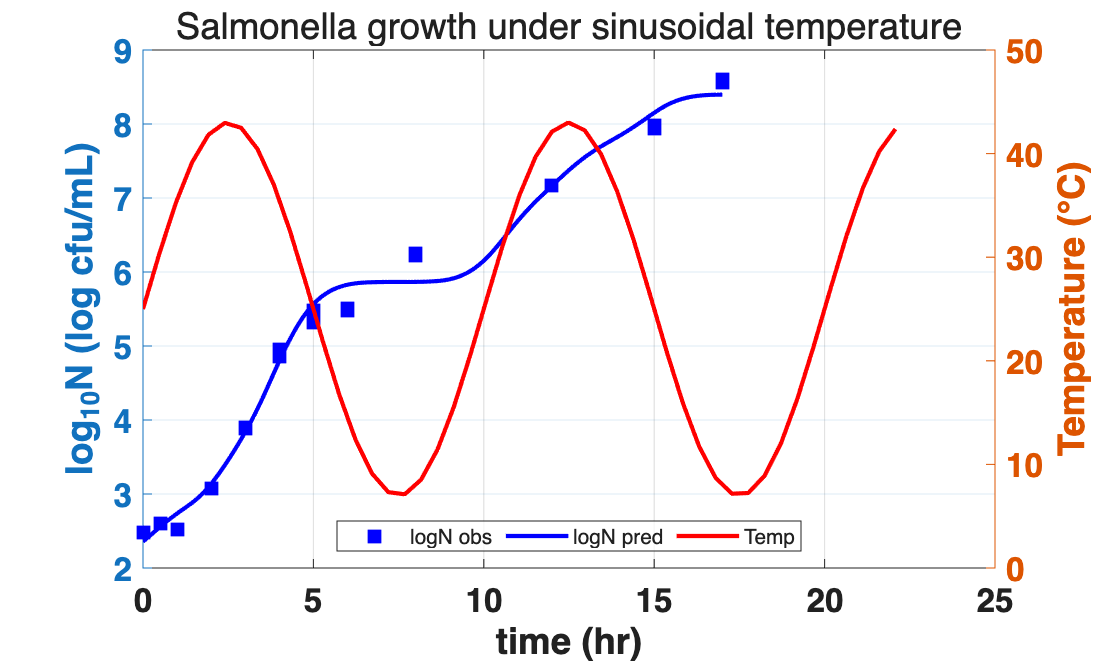
\includegraphics[width=\linewidth]{fig07_dual_axis_logN_temp.png}
				\caption{Fig 1. Dual-axis: $\log_{10} N$ and $T$ vs.\ time}
			\end{figure}
		\end{column}
	\end{columns}
\end{frame}

% ============================================================
% Slide 5: Forward Problem — Initial Guess
% ============================================================
\section{Forward Problem}
\begin{frame}
	\frametitle{Forward Problem — Initial Guess}
	\begin{columns}[T]
		\begin{column}{0.4\textwidth}
			\begin{itemize}
				\item All 7 parameter guesses from literature (Gumudavelli et al., 2007)
				\item ODE solved with \texttt{ode45}
				\item Temperature interpolated via \texttt{interp1}
			\end{itemize}
		\end{column}
		\begin{column}{0.58\textwidth}
			\begin{figure}
				\centering
				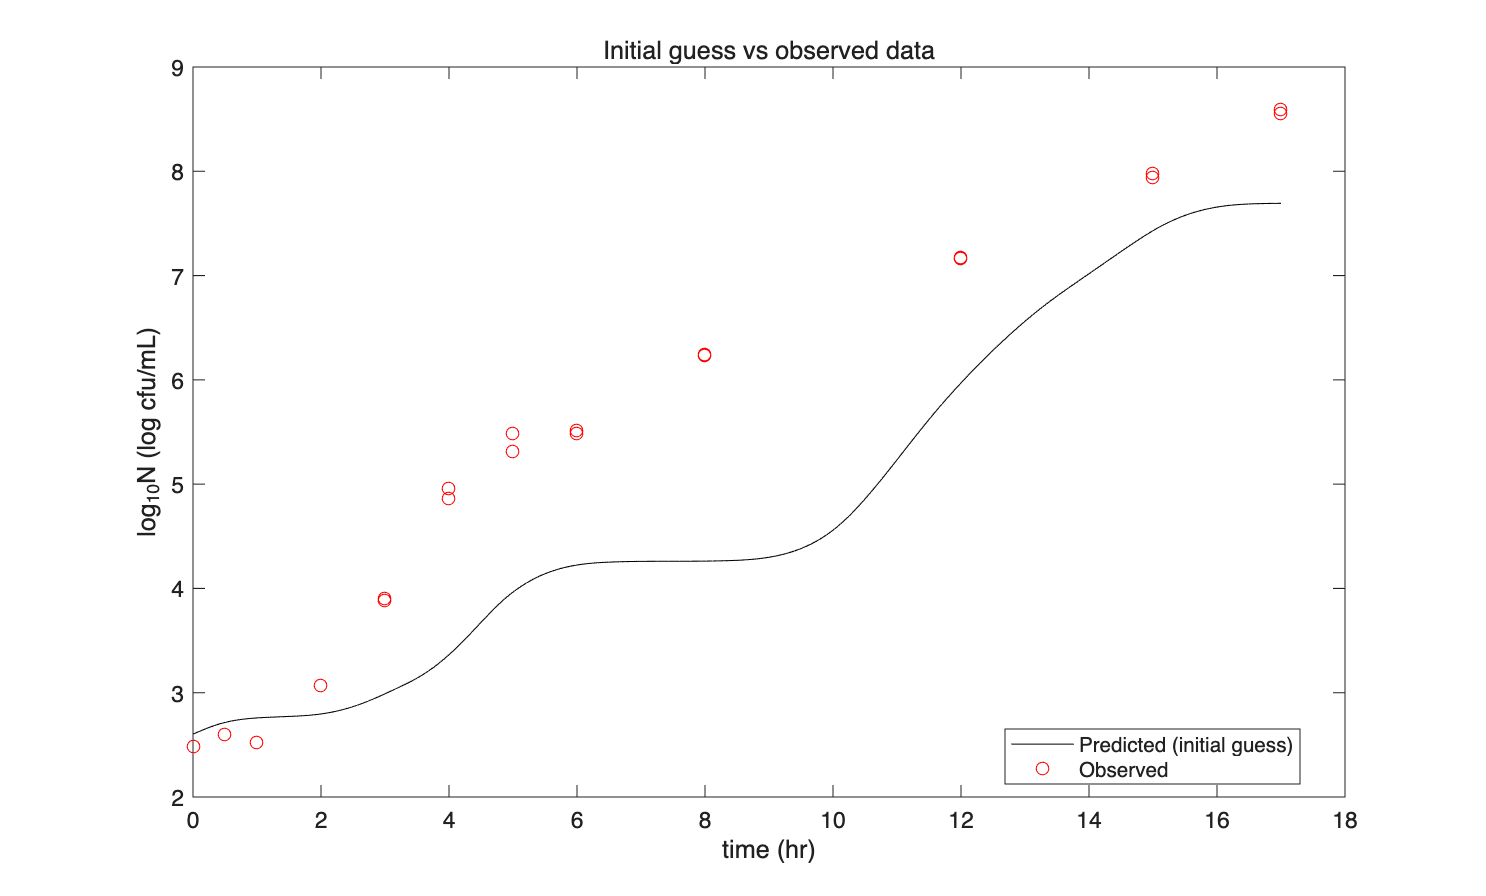
\includegraphics[width=\linewidth]{fig01_initial_guess_vs_data.png}
				\caption{Fig 2. Initial guess vs.\ observed data}
			\end{figure}
		\end{column}
	\end{columns}
\end{frame}

% ============================================================
% Slide 6: SSC Analysis — All 7 Parameters
% ============================================================
\section{Parameter Selection}
\begin{frame}
	\frametitle{SSC Analysis — All 7 Parameters (Step 1)}
	\begin{columns}[T]
		\begin{column}{0.28\textwidth}
			\scriptsize
			\textbf{Max$|$SSC$|$}:
			\vspace{0.2em}
			\begin{table}[ht]
				\centering
				\scriptsize
				\begin{tabular}{cc}
					\toprule
					Param & Max$|$SSC$|$ \\
					\midrule
					A & 2.61 \\
					C & 5.11 \\
					M & 5.45 \\
					a & 2.20 \\
					b & \textbf{0.88} \\
					$T_{\min}$ & \textbf{0.83} \\
					$T_{\max}$ & 9.02 \\
					\bottomrule
				\end{tabular}
			\end{table}
			\vspace{0.1em}
			\begin{block}{\scriptsize Decision}
				\tiny $T_{\min}$ (0.83) and $b$ (0.88): lowest SSC $\Rightarrow$ \textbf{fix}: $T_{\min}\!=\!6\,{}^{\circ}\text{C}$, $b\!=\!0.275$.
			\end{block}
		\end{column}
		\begin{column}{0.70\textwidth}
			\begin{figure}
				\centering
				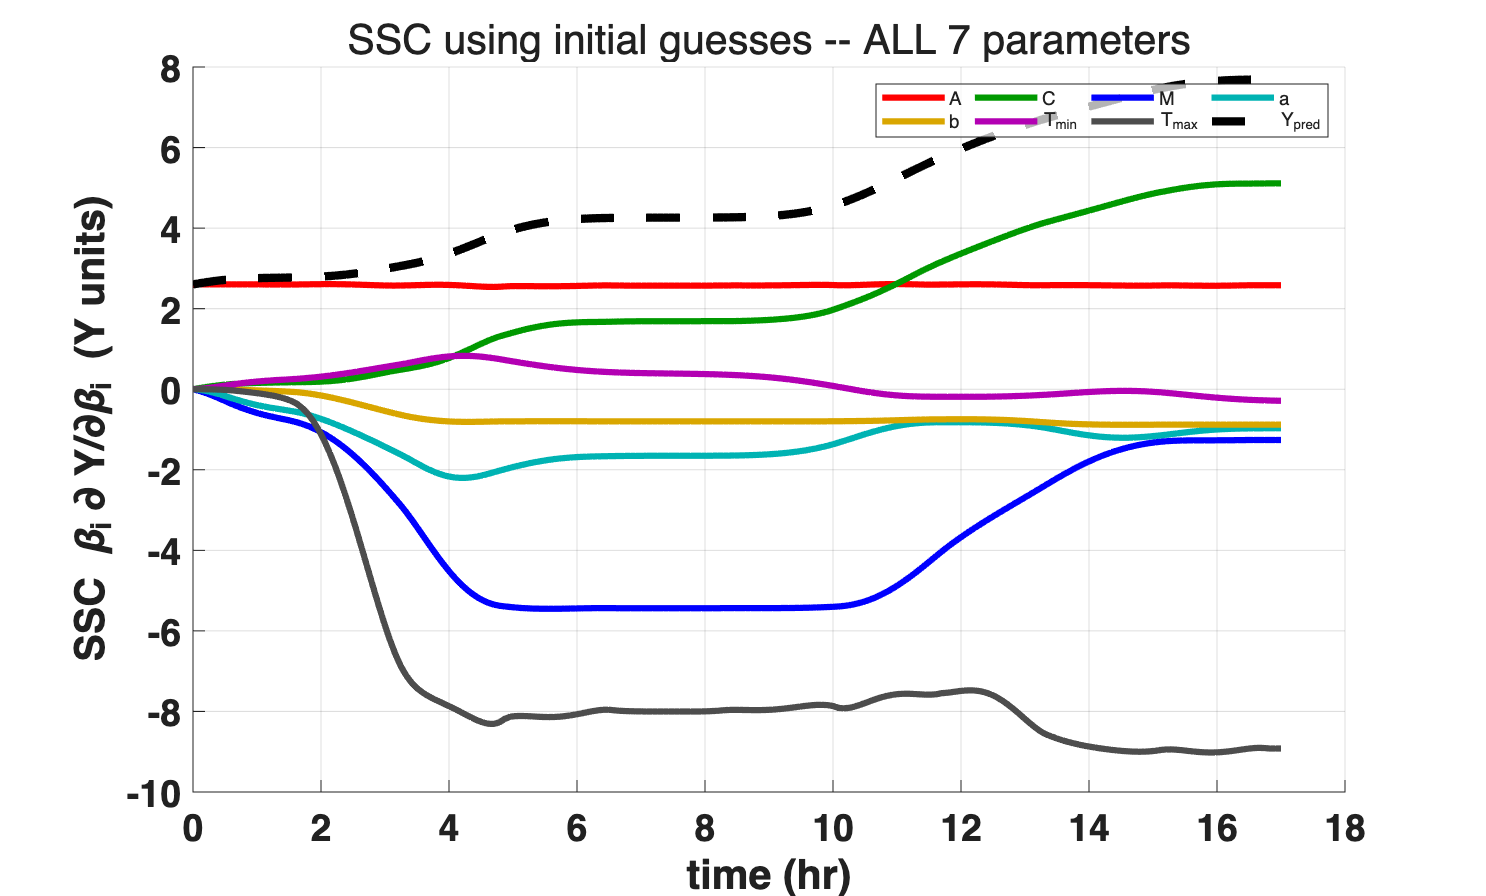
\includegraphics[width=0.92\linewidth]{fig02_SSC_7params.png}
				\caption{Fig 3. SSC for all 7 parameters}
			\end{figure}
		\end{column}
	\end{columns}
\end{frame}

% ============================================================
% Slide 7: Round 1 — Estimate 5 Parameters
% ============================================================
\begin{frame}
	\frametitle{Round 1 — Estimate 5 Parameters $[A, C, M, a, T_{\max}]$}
	\begin{columns}[T]
		\begin{column}{0.38\textwidth}
			\begin{itemize}
				\item Fixed: $T_{\min} = 6\,{}^{\circ}\text{C}$, $b = 0.275$
				\item Estimated: $A, C, M, a, T_{\max}$ ($p = 5$)
			\end{itemize}
		\end{column}
		\begin{column}{0.60\textwidth}
			\begin{figure}
				\centering
				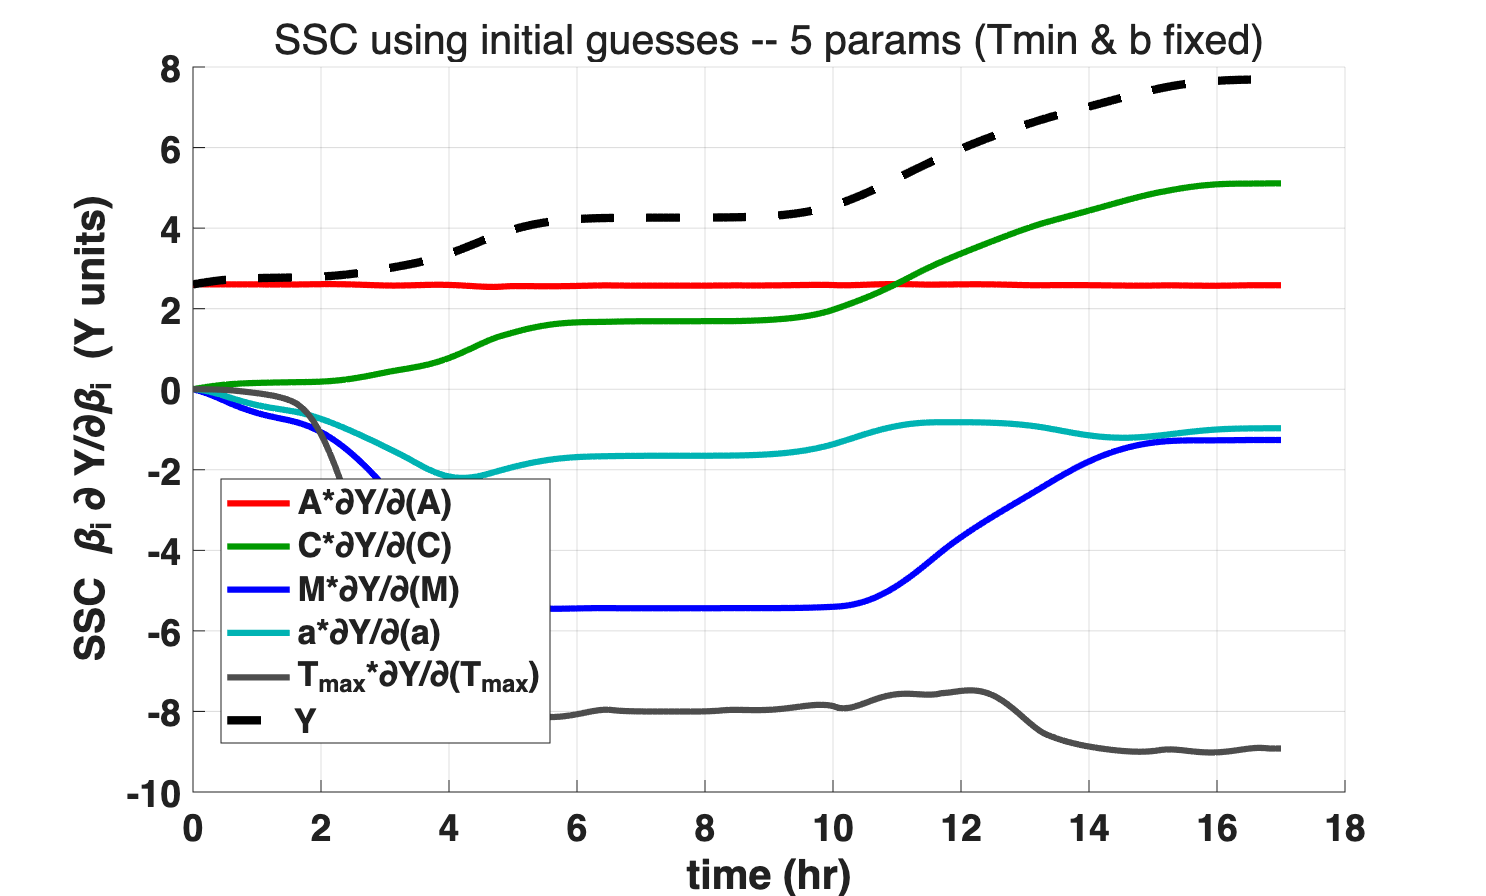
\includegraphics[width=\linewidth]{fig04_SSC_5params_round1.png}
				\caption{Fig 4. SSC with initial guesses (5 params)}
			\end{figure}
		\end{column}
	\end{columns}
\end{frame}

% ============================================================
% Slide 8: Round 1 Results & Parameter Selection Step 2
% ============================================================
\begin{frame}
	\frametitle{Round 1 Results \& Parameter Selection Step 2}
	\begin{columns}[T]
		\begin{column}{0.45\textwidth}
			\begin{itemize}
				\footnotesize
				\item \texttt{nlinfit} OLS estimation (5 params): $[A,C,M,a,T_{\max}]$
				\item $\text{cond}(\mathbf{J}) = 1.92\times 10^6$ — still ill-conditioned
				\item Correlation matrix: $M$--$a$ ($R=-0.994$), $C$--$T_{\max}$ ($R=-0.991$)
			\end{itemize}
			\vspace{0.2em}
			\begin{alertblock}{\footnotesize Key Finding}
				\scriptsize $a$ and $M$ are highly collinear: SSC shapes nearly proportional $\Rightarrow$ one must be fixed.
			\end{alertblock}
			\begin{block}{\footnotesize Decision}
				\scriptsize Fix $a$ at Round 1 estimate $\Rightarrow$ reduce to \textbf{4 parameters} $[A,C,M,T_{\max}]$.
			\end{block}
		\end{column}
		\begin{column}{0.53\textwidth}
			\begin{figure}
				\centering
				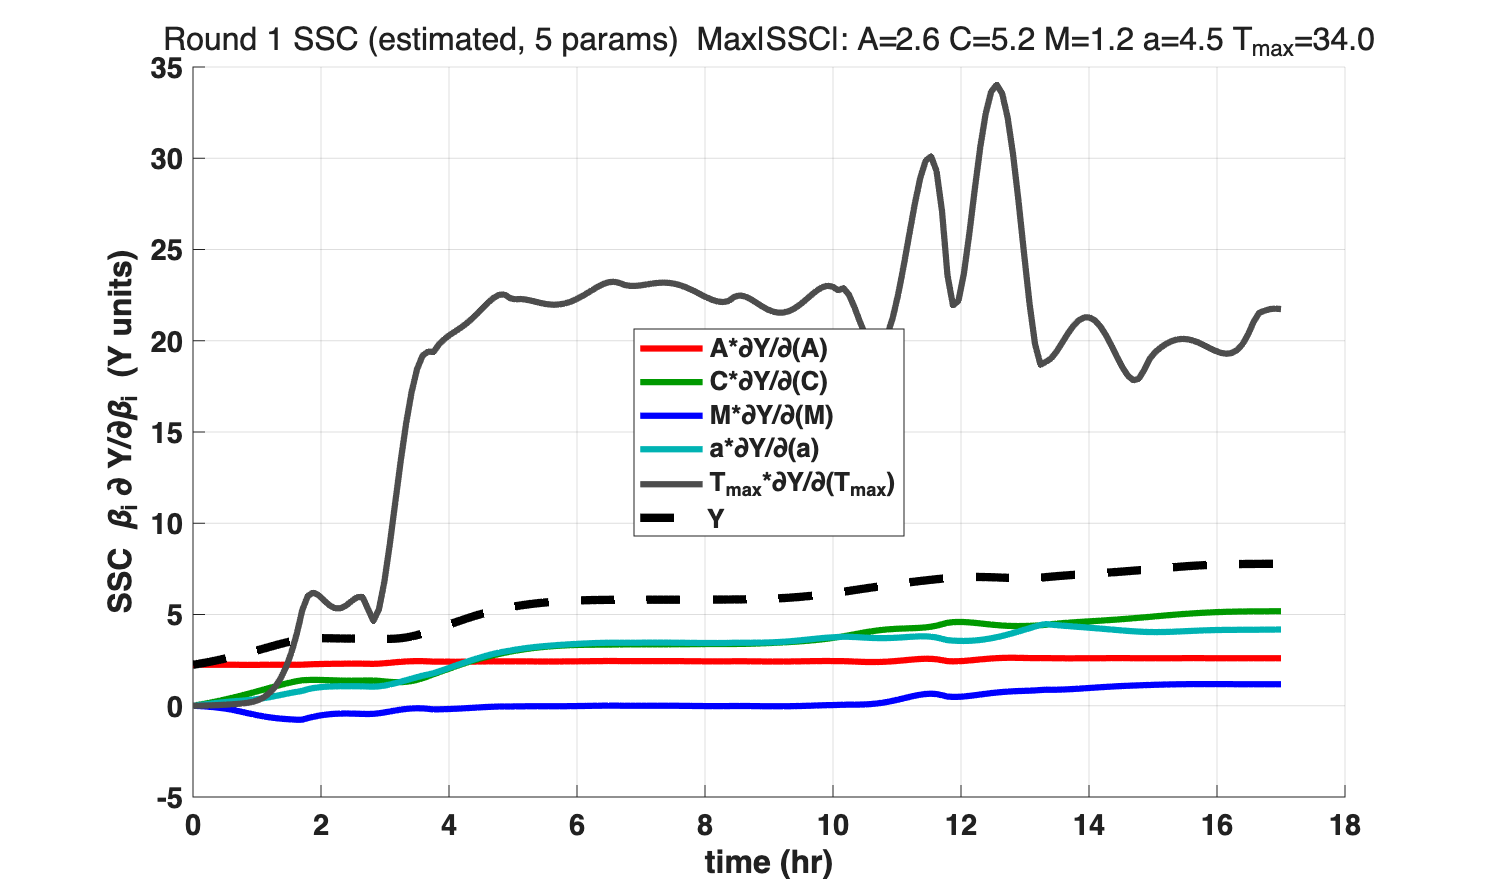
\includegraphics[width=\linewidth]{fig05_SSC_5params_estimated.png}
				\caption{Fig 5. SSC at estimated values (5 params)}
			\end{figure}
		\end{column}
	\end{columns}
\end{frame}

% ============================================================
% Slide 9: Parameter Selection Summary
% ============================================================
\begin{frame}
	\frametitle{Parameter Selection Summary}
	\begin{table}[ht]
		\centering
		\footnotesize
		\begin{tabular}{ccccc}
			\toprule
			Parameter & Max$|$SSC$|$ & Identifiable? & Action & Value Used \\
			\midrule
			A & 2.61 & \checkmark Yes & \textbf{Estimate} & OLS result \\
			C & 5.11 & \checkmark Yes & \textbf{Estimate} & OLS result \\
			M & 5.45 & \checkmark Yes & \textbf{Estimate} & OLS result \\
			$T_{\max}$ & 9.02 & \checkmark Yes & \textbf{Estimate} & OLS result \\
			$a$ & 2.20 & $\triangle$ Collinear w/ $M$ & Fix (Round 1 est.) & from Round 1 \\
			$b$ & 0.88 & $\times$ Low SSC & Fix (literature) & $0.275\,{}^{\circ}\text{C}^{-1}$ \\
			$T_{\min}$ & 0.83 & $\times$ Lowest SSC & Fix (literature) & $6\,{}^{\circ}\text{C}$ \\
			\bottomrule
		\end{tabular}
	\end{table}
	\vspace{0.3em}
	\begin{itemize}
		\item \textbf{Stepwise elimination}: $7 \to 5$ (fix $T_{\min}$, $b$) $\to 4$ (fix $a$)
		\item \textbf{Final estimable parameters}: $[A, C, M, T_{\max}]$, $\text{cond}(\mathbf{J}) = 293 \ll 10^6$ ✓
		\item SSC magnitude + collinearity check (ratio plot + $\text{cond}(\mathbf{J})$) together determine parameter selection
	\end{itemize}
\end{frame}

% ============================================================
% Slide 10: OLS Inverse Problem — Final Results (4 params)
% ============================================================
\section{OLS Results}
\begin{frame}
	\frametitle{OLS Inverse Problem — Final Results ($[A, C, M, T_{\max}]$)}
	\begin{table}[ht]
		\centering
		\footnotesize
		\begin{tabular}{ccccc}
			\toprule
			Param & Estimate & $\sigma$ & Rel Err & 95\% CI \\
			\midrule
			$A$ & 2.244 & 0.122 & 5.5\% & [1.985,\ 2.504] \\
			$C$ & 13.387 & 0.519 & 3.9\% & [12.29,\ 14.49] \\
			$M$ & 3.529 & 0.023 & 0.7\% & [3.479,\ 3.578] \\
			$T_{\max}$ & 41.651 & 0.022 & 0.05\% & [41.60,\ 41.70] \\
			\bottomrule
		\end{tabular}
	\end{table}
	\vspace{0.1em}
	\begin{itemize}
		\item Fixed: $T_{\min}=6\,{}^{\circ}\text{C}$,\ $b=0.275$,\ $a=3.6\times10^{-4}$ (Round 1 est.)
		\item $\text{cond}(\mathbf{J}) = 293 \ll 10^6$ ✓\quad RMSE $= 0.367$\quad relRMSE $= 6.3\%$\quad $R^2 = 0.972$
		\item Correlation: $C$--$T_{\max}$ ($R=-0.990$), $A$--$M$ ($R=-0.956$) — correlated but distinguishable
	\end{itemize}
\end{frame}

% ============================================================
% Slide 11: Fitted Curve with CB and PB
% ============================================================
\begin{frame}
	\frametitle{Fitted Curve with Asymptotic CB and PB}
	\begin{figure}[ht]
		\centering
		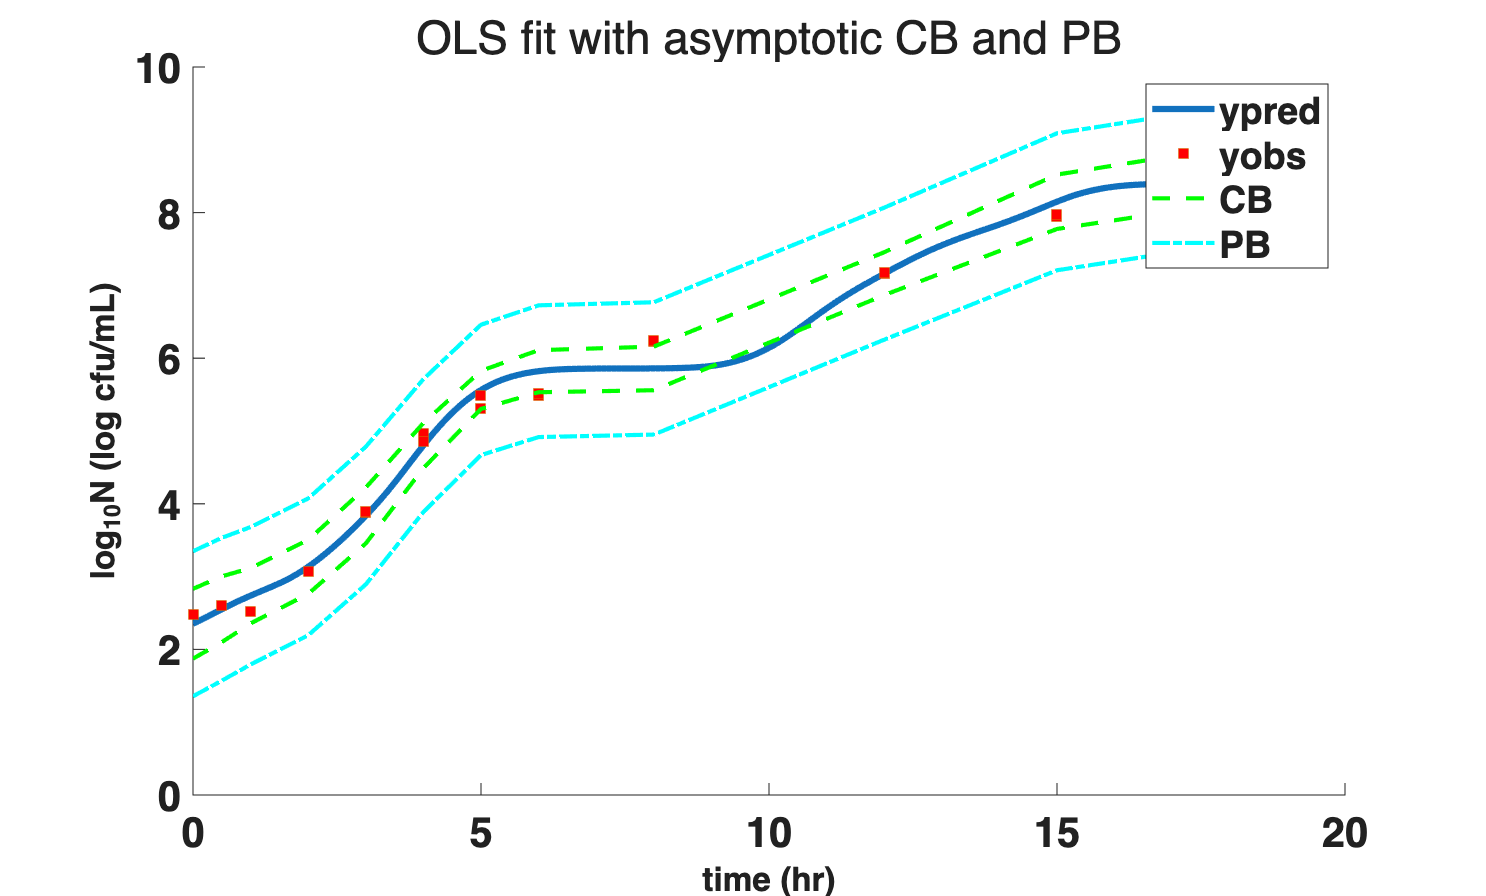
\includegraphics[width=0.65\linewidth]{fig06_OLS_fit_CB_PB.png}
		\caption{Fig 6. OLS fit with 95\% simultaneous confidence bands (CB) and prediction bands (PB)}
	\end{figure}
\end{frame}

% ============================================================
% Slide 12: Residual Analysis
% ============================================================
\section{Model Diagnostics}
\begin{frame}
	\frametitle{Residual Analysis}
	\begin{columns}[T]
		\begin{column}{0.35\textwidth}
			\begin{figure}
				\centering
				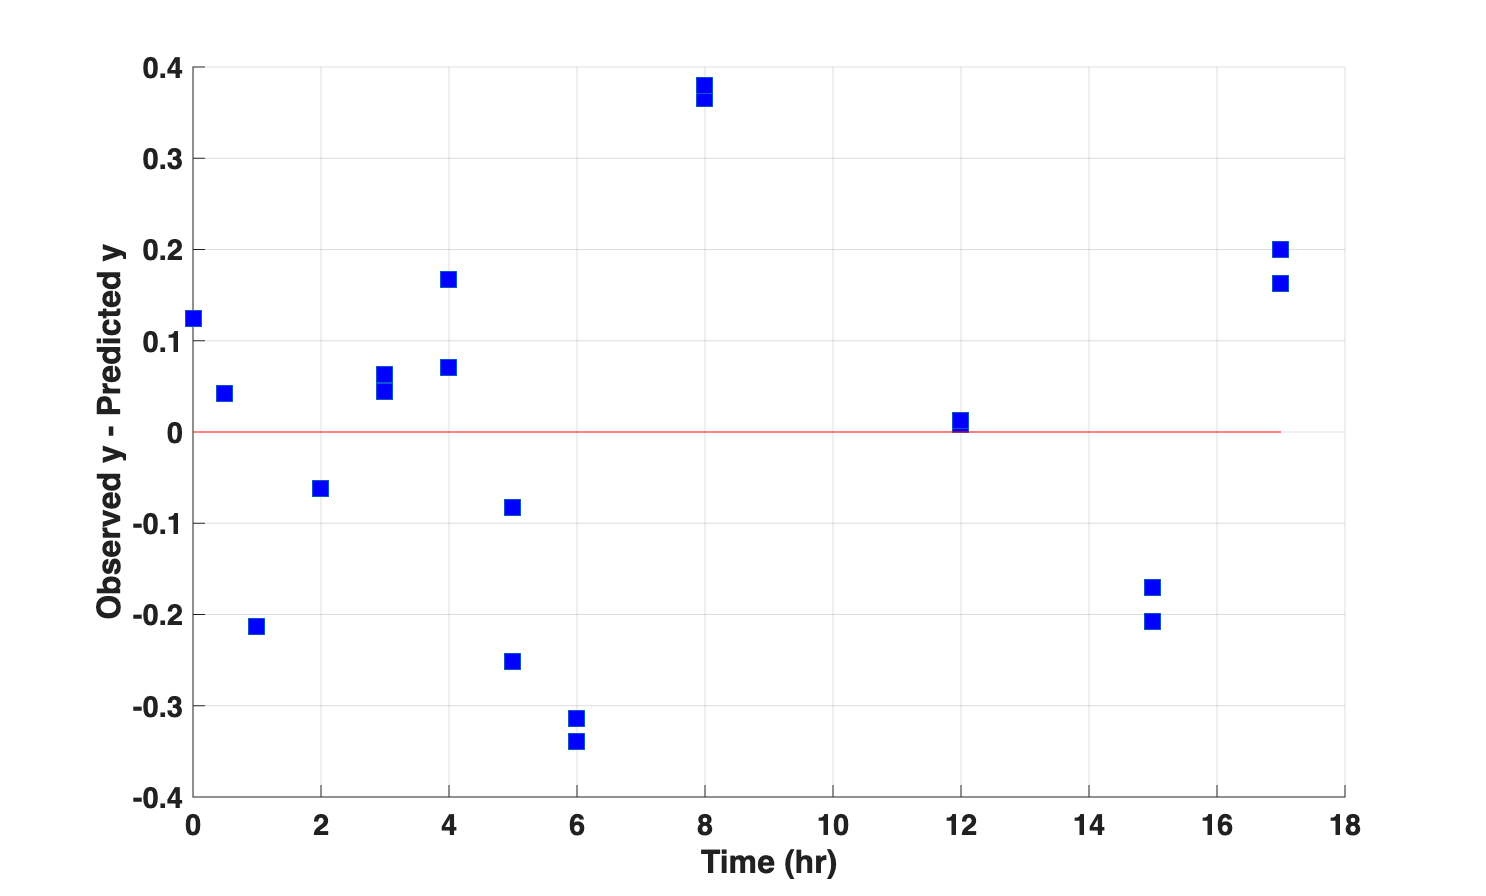
\includegraphics[width=\linewidth]{fig08_residual_scatter.png}
				\caption{Fig 7. Residual scatter}
			\end{figure}
		\end{column}
		\begin{column}{0.35\textwidth}
			\begin{figure}
				\centering
				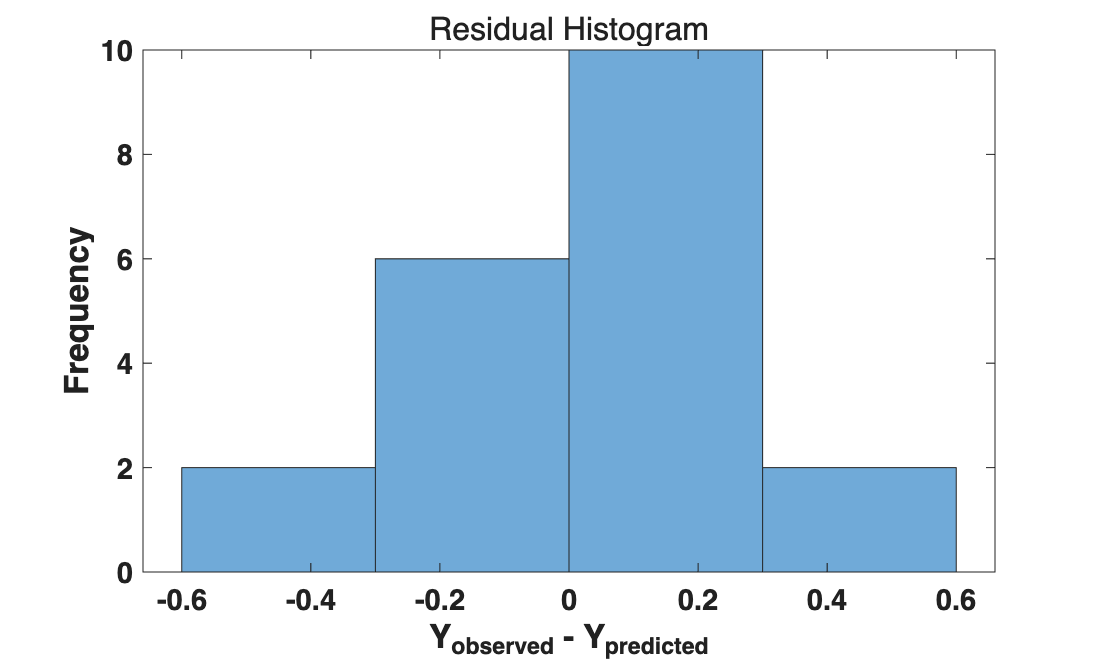
\includegraphics[width=\linewidth]{fig09_residual_histogram.png}
				\caption{Fig 8. Residual histogram}
			\end{figure}
		\end{column}
		\begin{column}{0.28\textwidth}
			\scriptsize
			\textbf{5 Assumptions}:
			\begin{enumerate}
				\item[\checkmark] Zero mean ($\approx 0.064$)
				\item[$\triangle$] Constant variance
				\item[$\triangle$] Uncorrelated (runs $= 6 < 10.5$)
				\item[\checkmark] Normality
				\item[\checkmark] Correct model
			\end{enumerate}
		\end{column}
	\end{columns}
\end{frame}

% ============================================================
% Slide 13: SSC Convergence — Round 2 Before vs After
% ============================================================
\begin{frame}
	\frametitle{SSC Convergence — Round 2 Before \& After Estimation}
	\begin{columns}[T]
		\begin{column}{0.48\textwidth}
			\begin{figure}
				\centering
				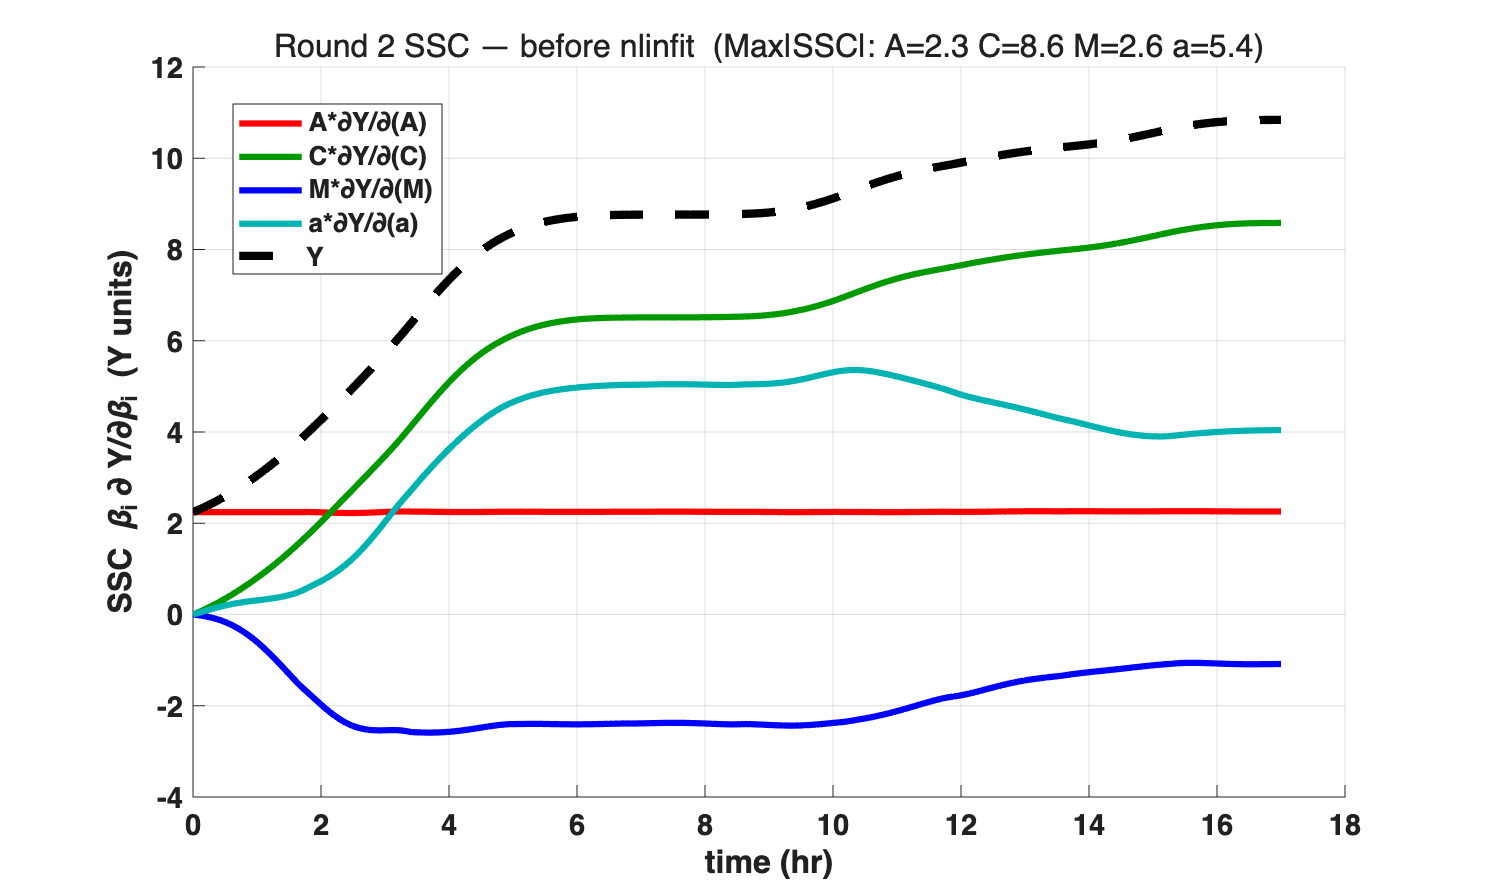
\includegraphics[width=\linewidth]{fig06a_SSC_4params_initial.png}
				\caption{Fig 9a. SSC using Round 1 estimates as initial guess}
			\end{figure}
		\end{column}
		\begin{column}{0.48\textwidth}
			\begin{figure}
				\centering
				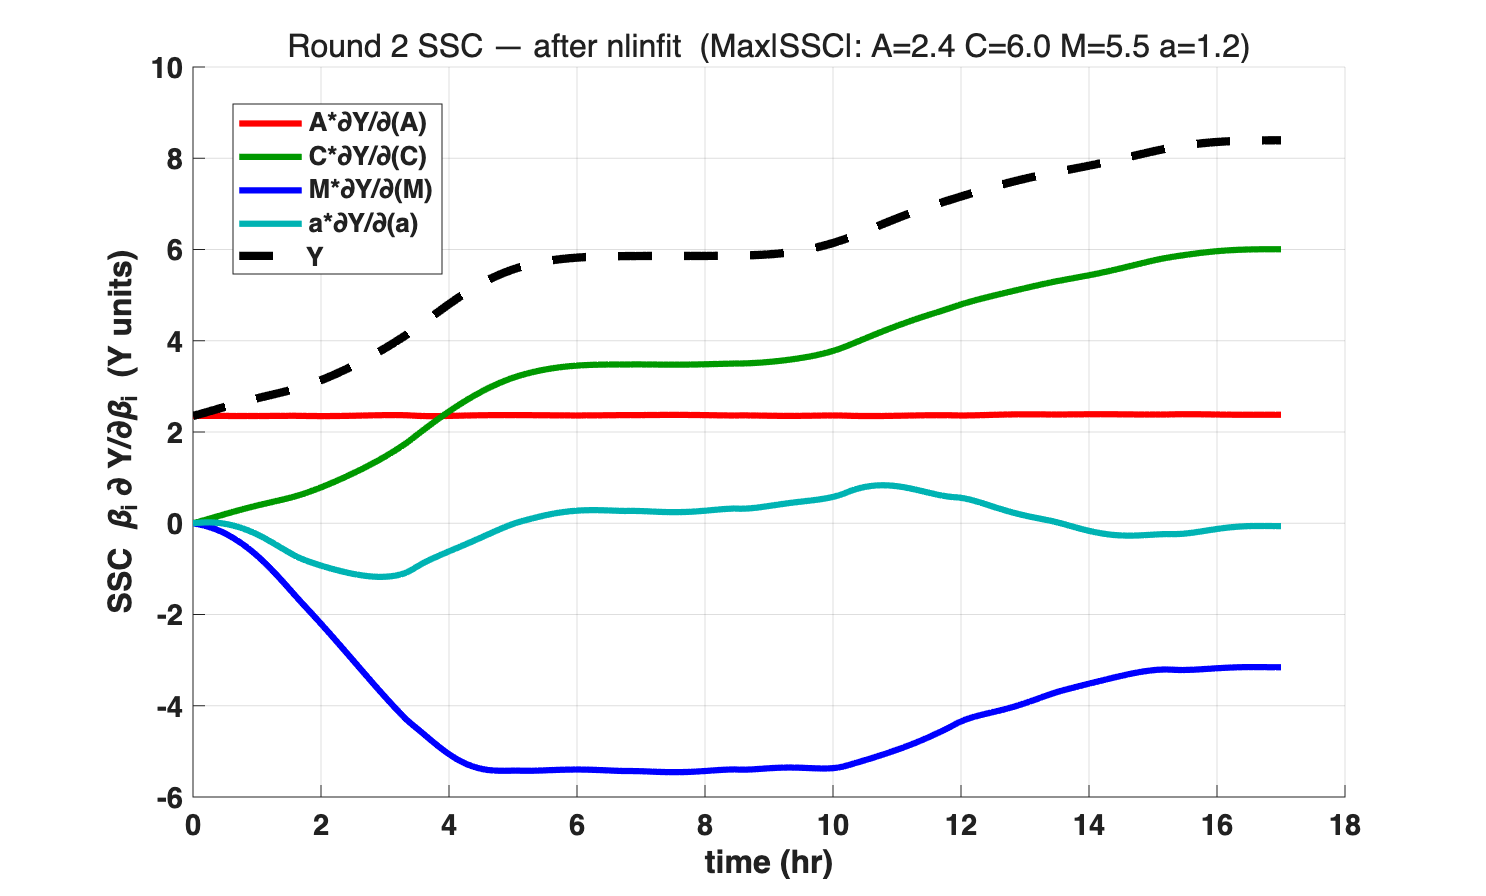
\includegraphics[width=\linewidth]{fig10_SSC_4params_final.png}
				\caption{Fig 9b. SSC after Round 2 OLS estimation}
			\end{figure}
		\end{column}
	\end{columns}
	\vspace{0.3em}
	\begin{block}{\small SSC Convergence Criterion}
		\small SSC shapes and magnitudes are consistent before and after Round 2 estimation $\Rightarrow$ parameter set is \textbf{stable and identifiable}; no further reduction needed.
	\end{block}
\end{frame}

% ============================================================
% Slide 14: Optimal Experimental Design
% ============================================================
\section{Optimal Experimental Design}
\begin{frame}
	\frametitle{Optimal Experimental Design}
	\begin{columns}[T]
		\begin{column}{0.4\textwidth}
			\vspace{1em}
			\begin{itemize}
				\item Equally-spaced \texttt{linspace} points (consistent with \texttt{inv\_soln5.m}); unscaled Jacobian $J=\partial Y/\partial\beta$
				\item Spikes at $n\approx27,34,48$: aliasing — equally-spaced points align with the $T_{\max}$ SSC peak at $t\approx12\,\text{hr}$
				\item For $n<22$: smooth increase of $\Delta$; $A$ has smallest $C_{ii}$ (most accurately determinable), $C$ most uncertain
			\end{itemize}
		\end{column}
		\begin{column}{0.58\textwidth}
			\begin{figure}
				\centering
				
\includegraphics[width=\linewidth]{fig11_OED_delta_Cii.png}
				\caption{Fig 10. $\Delta$ criterion and $C_{ii}$ vs.\ data points}
			\end{figure}
		\end{column}
	\end{columns}
\end{frame}

% ============================================================
% Slide 15: Bootstrapping of Residuals
% ============================================================
\section{Bootstrapping}
\begin{frame}
	\frametitle{Bootstrapping of Residuals}
	\begin{columns}[T]
		\begin{column}{0.45\textwidth}
			\footnotesize
			1000 bootstrap iterations (residual resampling), 1000/1000 valid.
			\vspace{0.3em}
			\begin{table}[ht]
				\centering
				\scriptsize
		\begin{tabular}{ccc}
				\toprule
				Param & Bootstrap 95\% CI & Asymptotic 95\% CI \\
				\midrule
				$A$ & [2.161,\ 2.511] & [1.985,\ 2.504] \\
				$C$ & [12.59,\ 14.61] & [12.29,\ 14.49] \\
				$M$ & [3.381,\ 3.612] & [3.479,\ 3.578] \\
				$T_{\max}$ & [41.29,\ 42.02] & [41.60,\ 41.70] \\
				\bottomrule
			\end{tabular}
			\end{table}
		\end{column}
		\begin{column}{0.53\textwidth}
			\begin{figure}
				\centering
				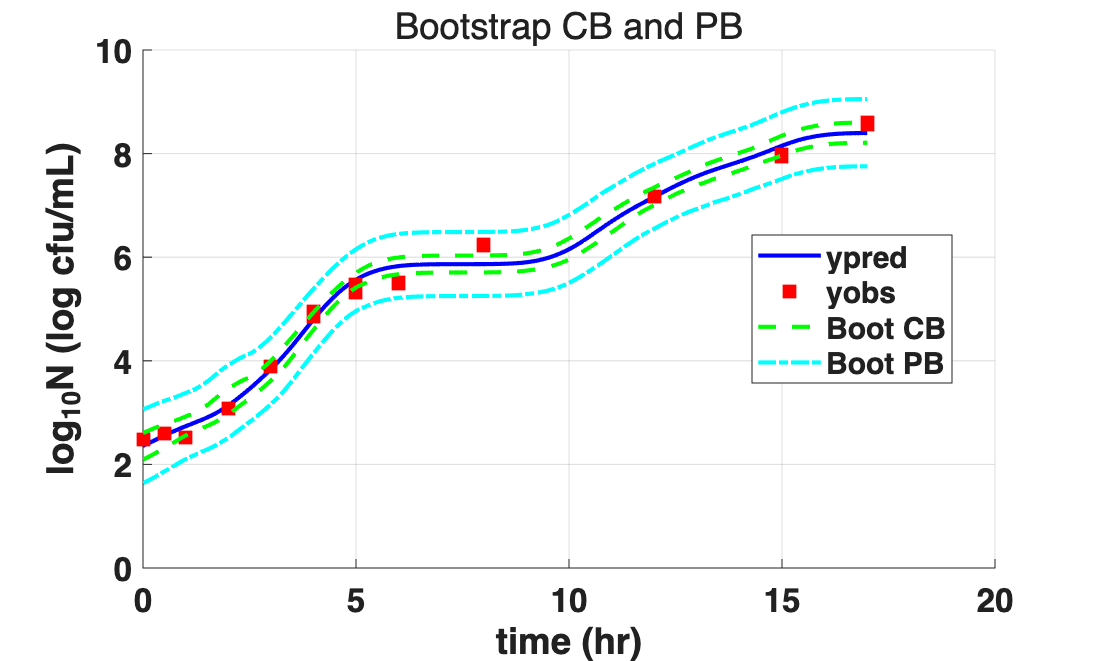
\includegraphics[width=\linewidth]{fig12_bootstrap_CB_PB.png}
				\caption{Fig 11. Bootstrap CB and PB}
			\end{figure}
		\end{column}
	\end{columns}
\end{frame}

% ============================================================
% Slide 16: Asymptotic vs Bootstrap Comparison
% ============================================================
\begin{frame}
	\frametitle{Asymptotic vs Bootstrap Comparison}
	\begin{table}[ht]
		\centering
		\begin{tabular}{lcc}
			\toprule
			Metric & Asymptotic & Bootstrap \\
			\midrule
			CB width (avg) & 1.044 & \textbf{0.372} \\
			PB width (avg) & 3.032 & \textbf{1.812} \\
			\bottomrule
		\end{tabular}
	\end{table}
	\vspace{0.5em}
	\begin{itemize}
		\item Bootstrap CB is $\mathbf{3\times}$ narrower; Bootstrap PB is $\mathbf{1.7\times}$ narrower
		\item Asymptotic method overestimates uncertainty due to $C$--$T_{\max}$ ($R=-0.990$) and $A$--$M$ ($R=-0.956$) correlations inflating the covariance matrix
		\item Bootstrap provides more realistic uncertainty quantification for this nonlinear problem
	\end{itemize}
\end{frame}

% ============================================================
% Slide 17: Conclusions
% ============================================================
\section{Conclusions}
\begin{frame}
	\frametitle{Conclusions}
	\begin{enumerate}
		\item Modified Gompertz model successfully predicts \textit{Salmonella} growth under sinusoidal temperature
		\item \textbf{Parameter selection}: SSC analysis + collinearity check $\Rightarrow$ identified $[A, C, M, T_{\max}]$ as estimable via stepwise elimination ($7\to5\to4$); fixed $T_{\min}$, $b$ (low SSC) and $a$ (collinear with $M$)
		\item Robust OLS fit achieved: $\text{cond}(\mathbf{J})=293$, relRMSE $= 6.3\%$, $R^2 = 0.972$; residual autocorrelation (runs test: 6 $<$ 10.5) suggests potential for model improvement
		\item Bootstrap CI are narrower than asymptotic CI $\Rightarrow$ asymptotic method overestimates uncertainty due to $C$--$T_{\max}$ ($R=-0.990$) and $A$--$M$ ($R=-0.956$) correlations
	\end{enumerate}
\end{frame}

% ============================================================
% References
% ============================================================
\section{References}
\begin{frame}[allowframebreaks]
    \frametitle{References}
    \reference
\end{frame}

\end{document}
